\chapter{Einführung}

% TODO : Quellenangaben
% gedankenstriche durch kommas ersetzen

Künstliche Intelligenz (KI) hat in den vergangenen Jahren einen rasanten
Aufschwung erlebt und beeinflusst heute nahezu alle Branchen, von der Medizin
über die Logistik bis hin zur Finanzwelt \cite{a_ki_2024, s_future_2024}. Auch
die Softwareentwicklung befindet sich im Umbruch: Moderne KI-Verfahren eröffnen
ein breites Spektrum neuer Einsatzfelder und verändern den Entwicklungsalltag
grundlegend \cite{siebert_generative_2024}. So unterstützt KI nicht mehr nur
bei der Automatisierung von Routinetätigkeiten wie Codierung und Testing,
sondern ermöglicht auch innovative Ansätze in der Fehlersuche,
Qualitätssicherung und Projektsteuerung \cite{a_ki_2024,
    siebert_generative_2024}.

Mit diesen Potenzialen gehen jedoch weitreichende Fragestellungen und
Herausforderungen einher. Neben technischen Aspekten wie Sicherheit, Robustheit
und Code-Qualität rücken gesellschaftliche Dimensionen zunehmend in den
Vordergrund, etwa die Frage nach ethischen Standards, Verantwortlichkeit und
der Veränderung des Berufsbilds von Softwareentwickler:innen
\cite{braun_ki_2024, schmitt_generative_2024, weisz_design_2024}. Insbesondere
der Siegeszug generativer KI, beispielsweise durch leistungsstarke Large
Language Models (LLMs), wirft komplexe Fragen zu Datenschutz, Fairness und der
Integration in bestehende Entwicklungsprozesse auf \cite{s_future_2024,
    weisz_design_2024}.

Vor diesem Hintergrund nimmt die vorliegende Arbeit eine umfassende Perspektive
ein: Ziel ist es, den Wandel der Softwareentwicklung unter dem Einfluss
generativer KI systematisch zu beleuchten und zentrale Chancen wie
Herausforderungen herauszuarbeiten. Im Mittelpunkt stehen dabei sowohl die
Auswirkungen auf die konkrete Arbeitssituation von Entwickler:innen als auch
die strategischen Implikationen für Unternehmen und Gesellschaft. Durch die
Verbindung von Literaturrecherche, Praxisbeispiel und kritischer Reflexion
sollen praxisrelevante Erkenntnisse sowie fundierte Handlungsempfehlungen
abgeleitet werden.

% Künstliche Intelligenz (KI) hat in den vergangenen Jahren einen rasanten
% Aufschwung erlebt und beeinflusst heute nahezu alle Branchen – von der Medizin
% über die Logistik bis hin zur Finanzwelt. Auch die Softwareentwicklung befindet
% sich im Umbruch: Moderne KI-Verfahren eröffnen ein breites Spektrum neuer
% Einsatzfelder und verändern den Entwicklungsalltag grundlegend. So unterstützt
% KI nicht mehr nur bei der Automatisierung von Routinetätigkeiten wie Codierung
% und Testing, sondern ermöglicht auch innovative Ansätze in der Fehlersuche,
% Qualitätssicherung und Projektsteuerung.

% Mit diesen Potenzialen gehen jedoch weitreichende Fragestellungen und
% Herausforderungen einher. Neben technischen Aspekten wie Sicherheit, Robustheit
% und Code-Qualität rücken gesellschaftliche Dimensionen zunehmend in den
% Vordergrund – etwa die Frage nach ethischen Standards, Verantwortlichkeit und
% der Veränderung des Berufsbilds von Softwareentwickler:innen. Insbesondere der
% Siegeszug generativer KI, beispielsweise durch leistungsstarke Large Language
% Models (LLMs), wirft komplexe Fragen zu Datenschutz, Fairness und der
% Integration in bestehende Entwicklungsprozesse auf.

% Vor diesem Hintergrund nimmt die vorliegende Arbeit eine umfassende Perspektive
% ein: Ziel ist es, den Wandel der Softwareentwicklung unter dem Einfluss
% generativer KI systematisch zu beleuchten und zentrale Chancen wie
% Herausforderungen herauszuarbeiten. Im Mittelpunkt stehen dabei sowohl die
% Auswirkungen auf die konkrete Arbeitssituation von Entwickler:innen als auch
% die strategischen Implikationen für Unternehmen und Gesellschaft. Durch die
% Verbindung von Literaturrecherche, Praxisbeispiel und kritischer Reflexion
% sollen praxisrelevante Erkenntnisse sowie fundierte Handlungsempfehlungen
% abgeleitet werden.

\section{Motivation}
% \subsection{Relevanz des Themas}
% % Diese Arbeit adressiert diese Problematik, indem sie die Chancen und Herausforderungen von KI in der Softwareentwicklung analysiert. Ziel ist es, sowohl wissenschaftliche als auch praktische Erkenntnisse zu gewinnen, die Unternehmen und Entwicklern helfen, informierte Entscheidungen über den Einsatz von KI-gestützten Technologien zu treffen.

% % Künstliche Intelligenz (KI) hat sich in den letzten Jahren als transformative Technologie in der Softwareentwicklung etabliert. Insbesondere generative KI-Modelle wie Large Language Models (LLMs) haben das Potenzial, Entwicklungsprozesse signifikant zu verändern. Die Automatisierung von Codegenerierung, Fehleranalyse und Softwarewartung führt zu einer gesteigerten Effizienz und ermöglicht es Entwicklern, sich auf konzeptionell anspruchsvollere Aufgaben zu konzentrieren.

% % Die zunehmende Integration von KI in den Softwareentwicklungsprozess eröffnet neue Möglichkeiten, birgt jedoch auch Herausforderungen. Während einige Studien eine gesteigerte Produktivität und Codequalität durch KI-gestützte Tools belegen, gibt es gleichzeitig Bedenken hinsichtlich Sicherheitsrisiken, algorithmischer Verzerrung und langfristigen Veränderungen in der Arbeitsweise von Entwicklern. Diese Gegensätze verdeutlichen die Notwendigkeit einer fundierten wissenschaftlichen Auseinandersetzung mit den Auswirkungen von KI auf die Softwareentwicklung.

% \subsection{Motivation}
% % Die zunehmende Verbreitung künstlicher Intelligenz (KI) in der Softwareentwicklung stellt sowohl Wissenschaft als auch Praxis vor bedeutende Herausforderungen und Chancen. Unternehmen integrieren KI-gestützte Tools in ihre Entwicklungsprozesse, um Produktivität und Codequalität zu steigern, doch der langfristige Einfluss dieser Technologie auf die Arbeitsweise von Softwareentwicklern ist noch nicht vollständig erforscht.

% % Besonders relevant ist die Frage, wie sich KI-gestützte Entwicklungsumgebungen auf traditionelle Softwareentwicklungspraktiken auswirken. Während einige Forschungen darauf hindeuten, dass KI-Tools repetitive Aufgaben reduzieren und Entwicklern mehr Raum für kreative Problemlösungen geben, bestehen weiterhin Unsicherheiten hinsichtlich der Verlässlichkeit der generierten Codevorschläge und möglicher ethischer Bedenken.

Die hohe Relevanz des Themas ergibt sich aus aktuellen Entwicklungen in
Forschung und Praxis: Immer mehr Unternehmen setzen auf KI-Technologien, um
Effizienzpotenziale und Innovationsschübe zu realisieren. Während generative
KI, etwa durch automatisierte Code-Generierung oder intelligente
Projektsteuerung enorme Fortschritte und Produktivitätsgewinne verspricht,
zeigen empirische Studien zugleich ein Spannungsverhältnis zwischen den
erhofften Vorteilen und realen Risiken wie Intransparenz, Sicherheitslücken und
ethischen Verzerrungen.

Nach aktuellen Schätzungen (Stand: 2025) erreicht der Softwaremarkt in
Deutschland ein Volumen von rund 31 Milliarden US-Dollar. Entwickler:innen
verbringen im Durchschnitt bis zu 17 Stunden pro Woche mit Wartungs- und
Routineaufgaben, ein Indikator dafür, wie groß der Bedarf an Automatisierung
und Qualitätsverbesserung in der Praxis ist. Genau hier setzt die generative KI
an: Tools wie GitHub Copilot können durch automatisierte
Boilerplate-Code-Generierung oder intelligente Code-Vervollständigung nicht nur
die Produktivität erhöhen, sondern auch das Fachkräftethema teilweise
entschärfen. Laut einer von Deloitte zitierten Studie lässt sich durch
KI-basierte Coding-Tools die für Routineaufgaben benötigte Entwicklerzeit um
bis zu 50\,\% reduzieren (vgl. \cite{s_future_2024}
\cite{siebert_generative_2024}).

Ein Beleg für die zunehmende wirtschaftliche Bedeutung ist der stetige Anstieg
der Investitionen in KI-Technologien für die Softwareentwicklung in den letzten
Jahren. Abbildung~\ref{fig:ki-investitionen} veranschaulicht diese Entwicklung
und unterstreicht, wie stark Unternehmen auf innovative KI-Lösungen setzen, um
sich Wettbewerbsvorteile zu sichern.

\begin{figure}[H]
    \centering
    \vspace{1em}
    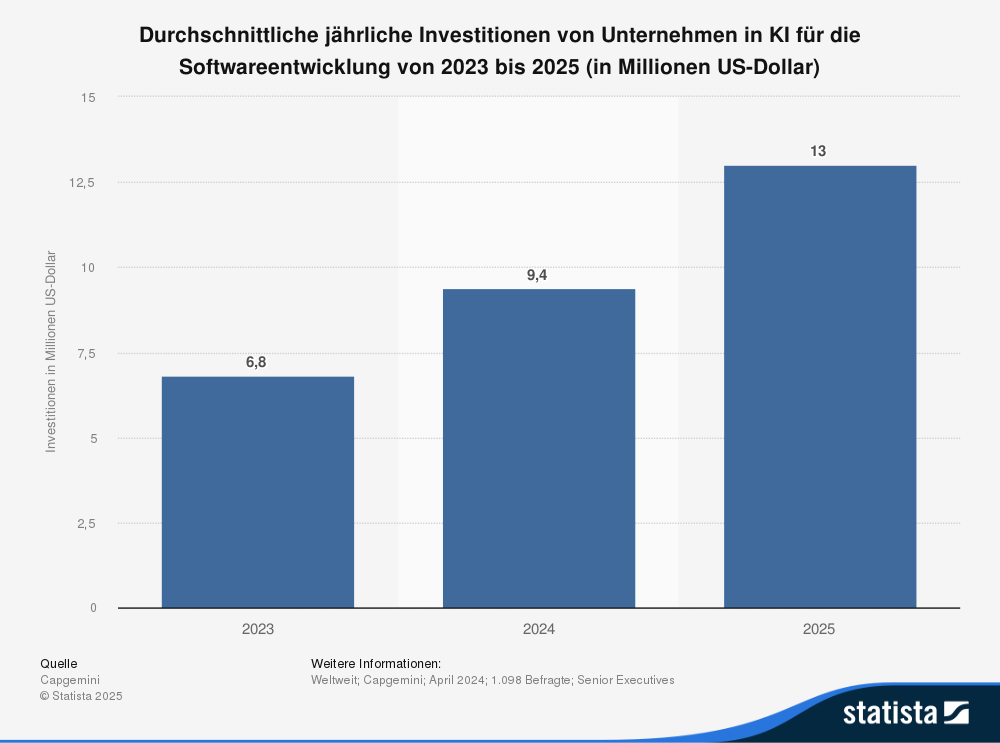
\includegraphics[width=0.7\textwidth]{images/abbildungen/statistic_id1481131_jaehrliche-investitionen-von-unternehmen-in-ki-fuer-softwareentwicklung-bis-2025.png}
    \caption{Jährliche Investitionen von Unternehmen in KI für Softwareentwicklung 2023–2025. Quelle: Capgemini~\cite{statista_ki_investitionen_2025}.}
    \label{fig:ki-investitionen}
\end{figure}

Allerdings werfen diese Entwicklungen auch kontroverse Fragen auf: In welchem
Maße verändert die zunehmende Abhängigkeit von KI-Tools die Rollen und
Kompetenzen von Softwareentwickler:innen? Wie kann sichergestellt werden, dass
durch KI-gestützte Automatisierung weiterhin qualitativ hochwertige, wartbare
und sichere Software entsteht~\cite{siebert_generative_2024}? Hinzu kommt, dass
die Softwareentwicklung durch agile Methoden wie Scrum oder Kanban bereits
stark dynamisiert ist. Die zusätzliche Integration von KI als Tool oder
„Co-Entwickler“ erhöht die Anforderungen an Prozessgestaltung, Rollenverteilung
und Qualitätsmanagement weiter.



\section{Zielsetzung und Fragestellungen}
Das Ziel dieser Arbeit ist es, die Auswirkungen von KI auf die Softwareentwicklung zu analysieren und praxisnahe Handlungsempfehlungen für Unternehmen und Entwickler abzuleiten. Dabei werden insbesondere folgende Forschungsfragen untersucht:

\begin{itemize}
    \item[FF-1] Wie verändert generative KI traditionelle Entwicklungspraktiken in der Softwareentwicklung?
    \item[FF-2] Welche spezifischen Herausforderungen entstehen durch KI-gestützte Softwareentwicklung hinsichtlich Sicherheit, Ethik und Code-Qualität?
    \item[FF-3] Wie kann Generative KI Softwareentwickler in einem agilen Entwicklungsprozess unterstützen? 
    \item[FF-4] Wie lassen sich bestehende generative KI-Tools (Cursor, GitHub Copilot, v0 etc.) in den Entwicklungsprozess einer React-Native-App integrieren, und welchen Einfluss hat das auf Entwicklungszeit und Code-Qualität?
    % \item[FF-4] Welche langfristigen Implikationen hat die Nutzung von KI auf die Rolle und Qualifikation von Softwareentwicklern?
    % \item[FF-5] Welche wirtschaftlichen und organisatorischen Auswirkungen hat die Integration von KI auf Softwareunternehmen und den Arbeitsmarkt?
\end{itemize}

Darüber hinaus wird ein praktisches Beispiel in Form einer React Native-App (Locals) angeführt, um zu untersuchen, wie bestehende generative KI-Tools (etwa Cursor, GitHub Copilot etc.) in einen realen Entwicklungsprozess integriert werden können.

\section{Methodik}

Die Arbeit folgt einem literaturbasierten, qualitativen Ansatz, um ein
umfassendes Bild der Potenziale und Herausforderungen generativer KI in der
Softwareentwicklung zu zeichnen. Ziel ist es, die aktuelle Forschungslage
systematisch zu erfassen, zu bewerten und praxisrelevante Schlüsse zu ziehen.
Die Methodik gliedert sich in folgende Schritte:

\begin{enumerate}
    % 1. punkt überprüfen: springer link & weiter quellen?
    \item \textbf{Literaturrecherche:} Umfassende Analyse wissenschaftlicher Publikationen aus IEEE Xplore, arXiv, SpringerLink sowie den in der Literaturdatenbank dieser Arbeit aufgeführten Fachquellen mit Fokus auf aktuelle Entwicklungen in der KI-gestützten Softwareentwicklung.
    \item \textbf{Kategorisierung der Forschungsthemen:} Strukturierte Erfassung und Gruppierung zentraler Themenfelder wie Automatisierung, Produktivität, Sicherheit und ethische Fragestellungen.
    \item \textbf{Vergleichende Analyse:} Systematischer Vergleich und Gegenüberstellung der Chancen und Herausforderungen auf Basis ausgewählter Studien und Fachbeiträge.
    \item \textbf{Synthese und Ableitung von Schlussfolgerungen:} Entwicklung praxisorientierter Empfehlungen für Unternehmen und Entwickler:innen zur Integration von KI in der Softwareentwicklung.
    \item \textbf{Praktische Demonstration:} Ergänzend zur Literaturauswertung wird ein Map-Screen (interaktive Kartenansicht) in der React Native-App „Locals“ exemplarisch implementiert. Dabei kommen verschiedene generative KI-Tools (u.a. Cursor, v0, GitHub Copilot) zum Einsatz, um die Unterstützung bei Code-Generierung, Testing und Qualitätsverbesserung zu evaluieren. Die gewonnenen Erkenntnisse aus diesem praktischen Teil werden systematisch mit den theoretischen Ergebnissen abgeglichen.
\end{enumerate}

Dieses methodische Vorgehen ermöglicht es, den aktuellen Forschungsstand
kritisch einzuordnen, praxisnahe Einblicke zu gewinnen und fundierte
Empfehlungen für die erfolgreiche Nutzung generativer KI in der
Softwareentwicklung abzuleiten.


% \section{Aufbau der Arbeit}
% Die Arbeit gliedert sich in folgende Kapitel:


\begin{itemize}
    \item \textbf{Kapitel 2:} Theoretische Grundlagen, in denen relevante Definitionen und Technologien der Künstlichen Intelligenz sowie Beispiele für generative KI-Tools vorgestellt werden.
    \item \textbf{Kapitel 3:} Chancen durch KI, mit einem Fokus auf Effizienzsteigerung und neuen Werkzeugen.
    \item \textbf{Kapitel 4:} Herausforderungen, einschließlich Sicherheits- und Datenschutzaspekten sowie ethischen Fragen.
    \item \textbf{Kapitel 5:} Fazit und Ausblick, mit einer Zusammenfassung der Ergebnisse und Handlungsempfehlungen.
\end{itemize}

\section{Abgrenzung}
Die Arbeit konzentriert sich auf die theoretische Analyse der Chancen und Herausforderungen von KI in der Softwareentwicklung. Folgende Aspekte werden bewusst ausgeklammert:

\begin{itemize}
    \item \textbf{Technische Implementierungen:} Es werden keine neuen KI-Modelle oder Algorithmen entwickelt.
    \item  \textbf{Empirische Studien:} Die Arbeit basiert auf einer literaturgestützten Analyse und führt keine Befragungen oder Experimente durch.
    \item \textbf{Rechtliche Rahmenbedingungen:} Eine detaillierte Untersuchung rechtlicher oder regulatorischer Aspekte wird nicht vorgenommen.
\end{itemize}

Obwohl ein begrenzter praktischer Teil in Form einer Funktionsimplementierung gezeigt wird, dient dieser in erster Linie als Proof of Concept. Eine umfassende empirische Evaluierung oder die Entwicklung eigener KI-Modelle findet nicht statt.

% Die Softwareentwicklung erlebt durch den Einsatz Künstlicher Intelligenz (KI) einen tiefgreifenden Wandel. Insbesondere generative KI-Modelle wie Large Language Models (LLMs) verändern etablierte Entwicklungspraktiken, indem sie Code generieren, automatisierte Tests durchführen und Entwicklungsprozesse effizienter gestalten. Diese Fortschritte werfen jedoch auch zentrale Fragen zur Sicherheit, zu ethischen Implikationen und zur langfristigen Rolle von Entwicklern auf.
%
% Erste Studien zeigen, dass KI-gestützte Tools signifikante Produktivitätssteigerungen ermöglichen, aber auch potenzielle Risiken wie Sicherheitslücken oder algorithmische Verzerrungen mit sich bringen. Daher ist es essenziell, eine fundierte wissenschaftliche Analyse durchzuführen, um Chancen und Herausforderungen umfassend zu bewerten.
%
% Diese Arbeit untersucht, wie KI-gestützte Softwareentwicklung die Produktivität und Qualität von Software beeinflusst, welche Herausforderungen sich daraus ergeben und welche praxisorientierten Anwendungen sich bereits abzeichnen. Dabei werden sowohl technologische als auch wirtschaftliche und gesellschaftliche Aspekte beleuchtet.
